\documentclass[letterpaper,10pt,twocolumn,titlepage]{article}

\usepackage{graphicx}                                        
\usepackage{amssymb}                                         
\usepackage{amsmath}                                         
\usepackage{amsthm}                                          

\usepackage{alltt}                                           
\usepackage{float}
\usepackage{color}
\usepackage{url}

\usepackage{balance}
\usepackage[TABBOTCAP, tight]{subfigure}
\usepackage{enumitem}
\usepackage{pstricks, pst-node}

\usepackage{geometry}
\usepackage{listings}
\geometry{textheight=8.5in, textwidth=6in}

%random comment

\newcommand{\cred}[1]{{\color{red}#1}}
\newcommand{\cblue}[1]{{\color{blue}#1}}

\usepackage{hyperref}
\usepackage{geometry}

\def\name{Balaji Ramani}

%% The following metadata will show up in the PDF properties
\hypersetup{
  colorlinks = true,
  urlcolor = black,
  pdfauthor = {\name},
  pdfkeywords = {cs311 ``operating systems'' files filesystem
I/O},
  pdftitle = {CS 311 Project 2:},
  pdfsubject = {CS 311 Project 2},
  pdfpagemode = UseNone
}

\begin{document}
\title{CS311: Operating Systems I - Assignment 2}
\author{Balaji Ramani}
\date{Feb 10, 2012}
\maketitle
\section{Commit logs}
\begin{center}
  \begin{tabular}{ | l | l | l | }
    \hline
    Time & Message & No of files \\ \hline
	2012/02/10 11:01 & comments and formatting & 1 \\ \hline
2012/02/10 10:48 & almost done & 1 \\ \hline
2012/02/09 06:58 & free malloced variables & 1 \\ \hline
2012/02/09 06:12 & first short at merge/suppressor & 1 \\ \hline
2012/02/09 02:12 & more stream related changes & 1 \\ \hline
2012/02/08 09:03 & add file streams & 1 \\ \hline
2012/02/08 07:36 & fix pipe issues and load sort in the children & 1 \\ \hline
2012/02/03 20:29 & spacing issues & 1 \\ \hline
2012/02/03 01:19 & writing parsed output to child's input & 1 \\ \hline
2012/02/02 23:26 & parser logic & 1 \\ \hline
2012/01/31 08:00 & HW2 - initial commit - basic structure & 1 \\ \hline
  \end{tabular}
\end{center}
\section{File size vs Time plot}
		\begin{figure}
			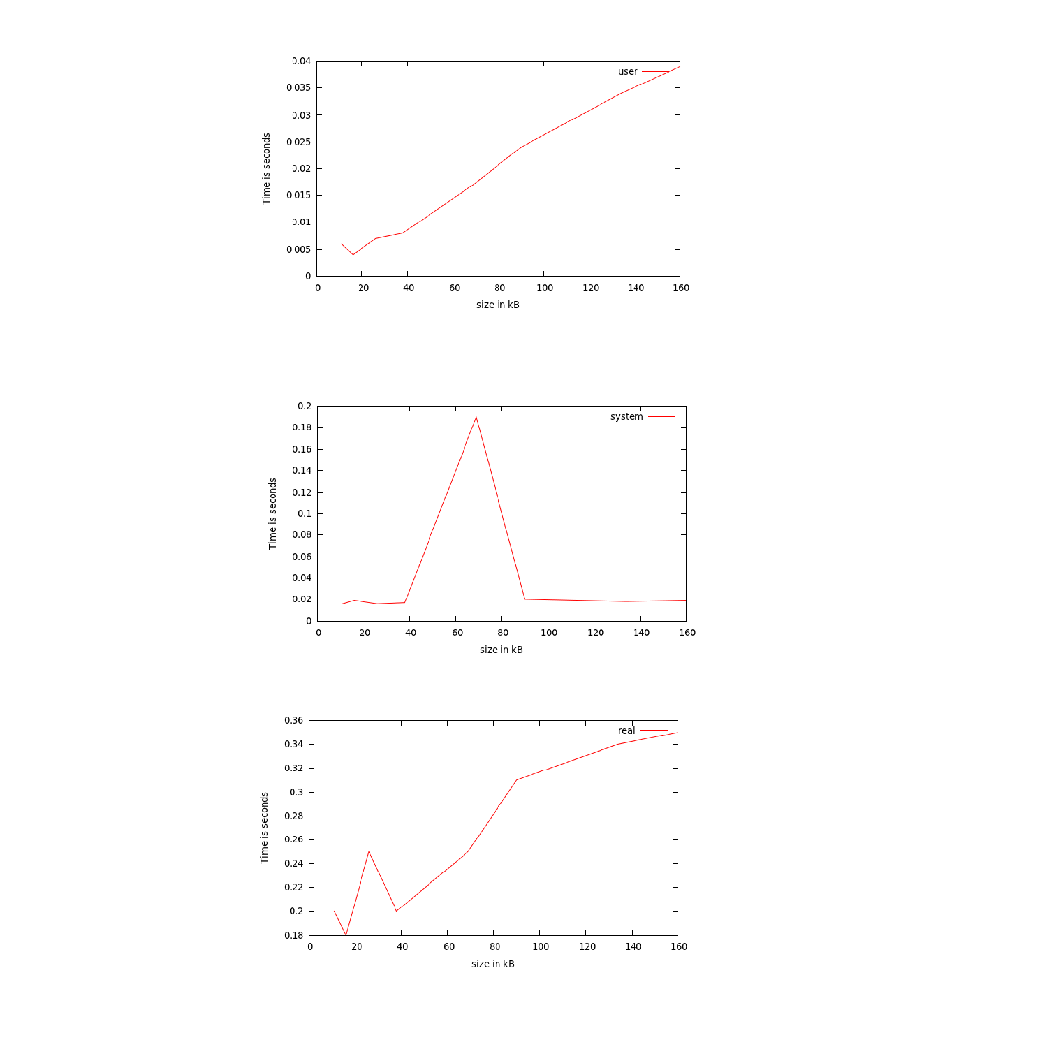
\includegraphics[scale=0.3]{graphs.eps}
		\end{figure}
\end{document}
